 
 
\documentclass[french]{spimufcphdthesis}
 

\usepackage[utf8]{inputenc}
\usepackage{enumitem}
\usepackage{float}

\declarethesis[Sous-titre]{Combinaison de SysML et Model Checker pour la Simulation et la Vérification Formelle}{14 Mars 2018}{Besan\c{c}on}{XXX}
 

\addauthor[karimboudaoude@gmail.com]{Karim}{Boudaoud}

\addjury{Incroyable}{Hulk}{Pr\'esident}{Professeur à l'Université de Gotham City}
 

\thesisabstract[french]{SysML est un langage de modélisation des systèmes rapidement émergeant comme une norme de facto utilisée pour les spécifications logicielles, les diagrammes de séquence UML fournissent une technique visuelle pour modéliser et dépeindre les comportements logiciels. Cependant, les diagrammes de séquence ne peuvent pas automatiquement analyser et vérifier les comportements logiciels dû au manque de sémantique stricte. Pour assurer la fiabilité du logiciel systèmes, une description du comportement et une approche de vérification formelle est proposé dans ce projet, qui utilise le diagramme de séquence SYSML et un modèle d'automate.
 
Premièrement, une relation complète est établie entre le diagramme de séquence et le réseau d'automates temporisés à partir de certaines règles de transformation.

Ensuite, suivant la base des règles prédéfinies, la transformation du modèle sera établie.

La vérification formelle peut être ensuite effectué pour vérifier les propriétés du domaine basées sur le langage TCTL comme étant une logique expressive non ambiguë avec un vérificateur de modèles automatisés (UPPAAL).

Notre proposition comble le fossé entre la modélisation visuelle et la modélisation formelle logiciel, ainsi qu’avancer l’étape de vérification le plus tôt possible dans le cycle de développement des systèmes hétérogène.

Notre approche a été évaluée sur un système de simulation d’ATM. L’étude de cas montre que cette approche proposée est efficace et efficiente dans le comportement, description et vérification formelle du logiciel.
}
 

\thesiskeywords[french]{SysML, Diagramme de Séquence , V\'erification Formelle , Automate Temporis\'e ,Modèle de transformation, UPPAAL}

\resetlaboratories


\addlaboratory{Laboratoire DISC}


\declareupmtheorem{mytheorem}{My Theorem}{List of my Theorems}


\begin{document}
 

\chapter*{Remerciements}
Nous ne pouvons pas laisser passer l’occasion de la présentation de ce rapport sans exprimer nos remerciements et notre gratitude à tous ceux qui ont bien voulu nous apporter l’assistance nécessaire au bon déroulement de ce projet.
Nous adressons nos sincères remerciements à notre encadrant, Messabihi Mohammed, pour l’attention et l’intérêt qu’il a porté à notre travail et pour ses multiples conseils et orientations tout au long de l'élaboration de ce projet.
Nous tenons aussi à témoigner notre reconnaissance envers tous nos collègues de travail pour toutes les discussions concernant ce sujet.

\tableofcontents


\mainmatter
 
\part{Contexte et Problématiques}
\chapter{Introduction}

 Les systèmes critiques temps réel deviennent de plus en plus complexes et exigeants un niveau de sûreté et de fiabilité très élevé. Cela nécessite l'utilisation des méthodes de spécification et de vérification dans la phase de conception pendant le cycle de développement de ces systèmes afin de réduire la notion d'erreur avant même de commencer l'implémentation ce qui permet le développement d'un système fiable, de réduire les coûts et de gagner du temps.
 
 
\section{Contexte}

Ce sujet est situé dans un contexte de recherche et développement pour la modélisation et la vérification
de  systèmes  hétérogènes  (par  exemple  des  systèmes  répartis  sur  des  plateformes  diverses  ou  des
logiciels  embarqués  sur  divers  matériels).   La  composition  souple  de  divers  composants  est  une
voie pour modéliser et construire de tels systèmes.  Cependant afin de les analyser et garantir leur
correction vis à vis des exigences, il faut formaliser les propriétés locales ou globales et les vérifier.

\section{Problématique}

\section{Objectifs}
Les objectifs de cette thèses sont :

\section{Organisation du mémoire}


\part{Chapitre 1}

\chapter{État de l'art}



\section{Langages de modélisation}

 Les langages de modélisation sont couramment utilisés pour spécifier, visualiser, stocker, documenter, et échanger des modèles de conception. Ils sont spécifiques au domaine et contiennent toutes les informations syntaxiques, sémantiques et de présentation concernant une application donnée dans un domaine. Différents langages de modélisation ont été définis par des organisations et des entreprises afin de cibler différents domaines tels que le développement web (WebML), télécommunications (TeD), matériel (HDL), logiciels, et plus récemment, les systèmes (UML). D'autres langages tels que IDEF ont été conçus pour un large éventail d'utilisations, y compris la modélisation fonctionnelle, la modélisation des données et la modélisation de résaux.
Bien que l’ingénierie des systèmes existe depuis plus de cinq décennies, jusqu'à récemment, il n'y avait pas de langage de modélisation dédié à cette discipline. Traditionnellement, les ingénieurs systèmes ont beaucoup travaillé sur la documentation pour exprimer les exigences système et, en l'absence d'une langue standard spécifique, ont utilisé différents langages de modélisation pour exprimer une solution de conception complète.
Cette diversité de techniques et d'approches a limité le travail coopératif et l'échange d’information. Parmi les langages de modélisation existants qui ont été utilisés par les systèmes ingénieurs, on peut citer HDL, IDEF et EFFBD. Afin de fournir une solution à ce problème, OMG et INCOSE, avec un certain nombre d'experts dans le domaine de l’ingénierie système, ont collaboré pour la construction d'un langage de modélisation standard pour IE.
UML, étant le langage de modélisation par excellence pour l'ingénierie logicielle, était le langage de choix destiné à la personnalisation à l'égard des besoins des ingénieurs systèmes. Cependant, UML 1.x s'est révélée inadéquate pour une telle utilisation et donc la révision en évolution de UML (c'est-à-dire, UML 2.0) a été publié, avec des fonctionnalités spéciales pour les ingénieurs systèmes. En avril 2006, une proposition pour un langage de modélisation standard pour la modélisation des systèmes, à savoir SysML, a été soumis à l'OMG, avec l'objectif d'aboutir à un processus de normalisation final.

\subsection{UML}

 Le langage de modélisation unifié (UML) est une modélisation visuelle à usage général langue dont la maintenance a été assumée par OMG depuis 1997. C'est le résultat de la fusion de trois notations majeures : la méthodologie de Grady Booch pour décrire un ensemble d'objets et leurs relations, la technique de modélisation des objets de James Rumbaugh (OMT), et la méthodologie de cas d'utilisation d'Ivar Jacobson.
Bien que UML ait été conçu à l'origine pour spécifier, visualiser et documenter systèmes logiciels, il peut également être appliqué à divers autres domaines tels que l’organisation des sociétés et processus d'affaires. UML a de nombreux avantages, il est largement accepté par de nombreux leaders de l'industrie, est non exclusif et extensible et est également commercialement soutenu par de nombreux outils et manuels. La norme UML a été révisé plusieurs fois et de nombreuses versions ont été publiées jusqu’à la version 2.5.1 publiée en 2018. 

\subsubsection{Metamodel UML}

 L'infrastructure définit les concepts de bas niveau dans UML et représente un métamodèle. La superstructure UML concerne la définition des éléments UML. Le document de la superstructure contient la description de la syntaxe UML, y compris les spécifications des diagrammes. Il définit 13 diagrammes qui peuvent être classés en deux catégories principales : diagrammes structurels et diagrammes comportementaux. Enfin, la spécification OCL définit une langue pour écrire des contraintes et des expressions dans les modèles UML.

\begin{figure}[H]
\begin{center}
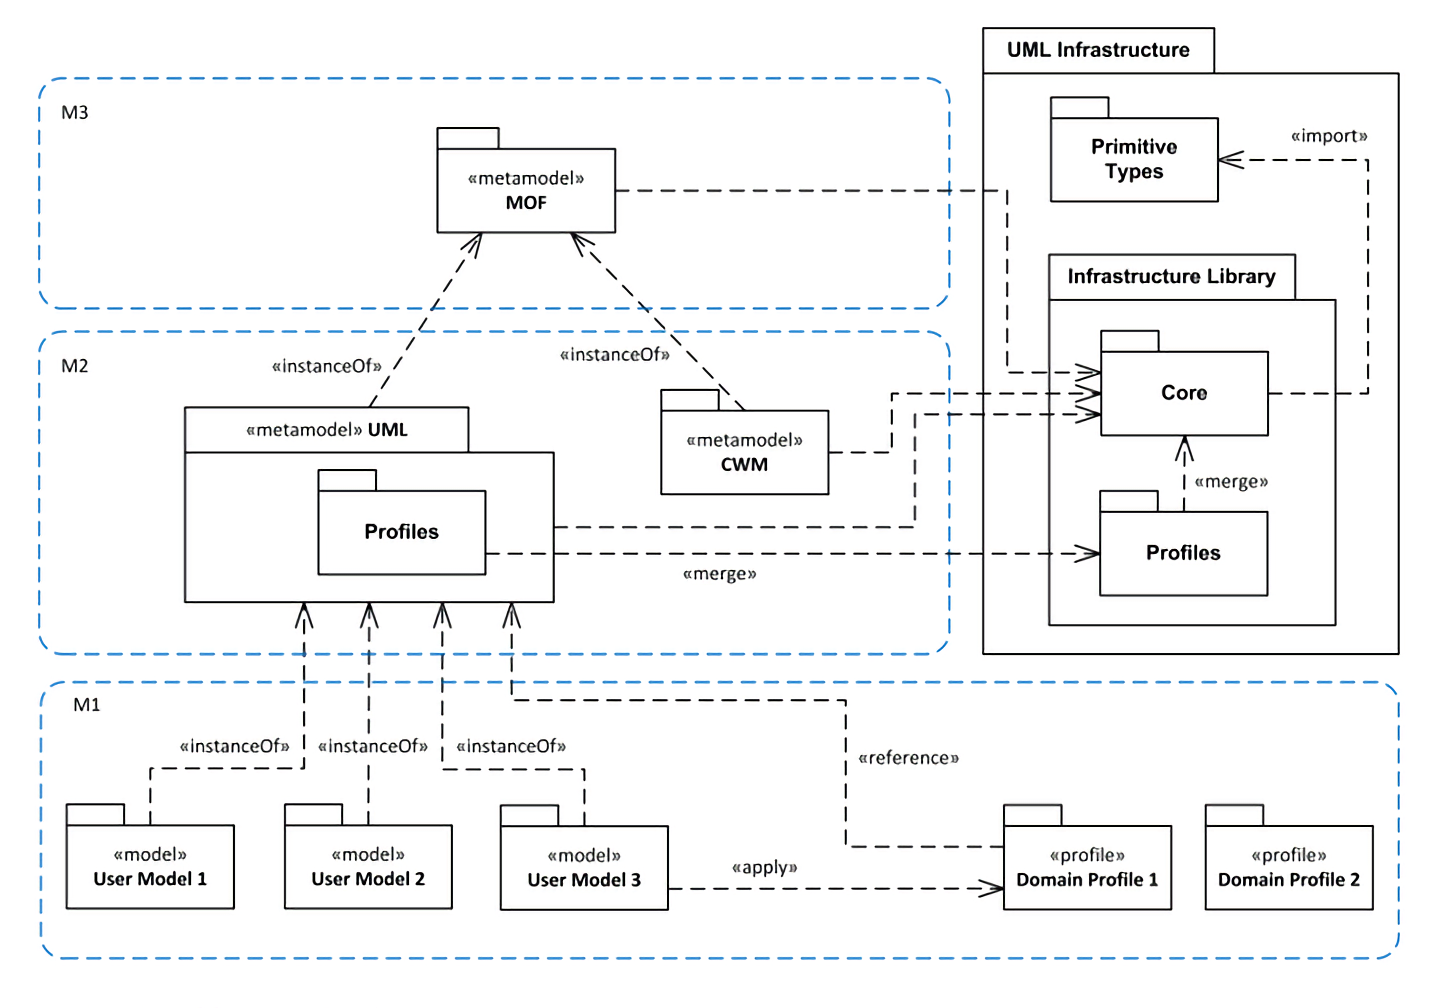
\includegraphics[scale=0.5]{figures/Metamodel.png}
\caption{Metamodel UML}
\label{UML_meta}
\end{center}
\end{figure}

\subsubsection{Architecture UML}

 Les diagrammes UML sont classés en deux catégories principales : structurelle et comportementale. Cette dernière catégorie comprend une catégorie de sous-ensembles appelée diagrammes d'interaction. La taxonomie des diagrammes est illustrée à la Fig \ref{UML_diag}.
Les diagrammes structurels modélisent les aspects statiques et les caractéristiques structurelles du système, tandis que les diagrammes comportementaux décrivent le comportement dynamique du système.
Les diagrammes structurels incluent le diagramme de classe, le diagramme de composants, le diagramme de structure composite, le diagramme de déploiement, le diagramme d’objet, et le diagramme de packages. 
Les diagrammes comportementaux incluent le diagramme d’activité, le diagramme de cas d'utilisation et le diagramme d’état machines. 
Les diagrammes d'interaction font partie de de la catégorie des diagrammes comportementaux car ils soulignent l'interaction entre les composants modélisés. Ils comprennent le diagramme de communication, le diagramme global d’interactions, le diagramme de séquence et le diagramme de temps. 
Les nouveaux diagrammes proposés dans UML 2.x sont le diagramme de structure composite, le diagramme global d’interactions et le diagramme de temps. En outre, d'autres diagrammes ont été étendus et modifiés depuis UML 1.x, à savoir, le diagramme d’activité, le diagramme d’état machine, le diagramme de séquence et le diagramme de communication.

\begin{figure}[H]
\begin{center}
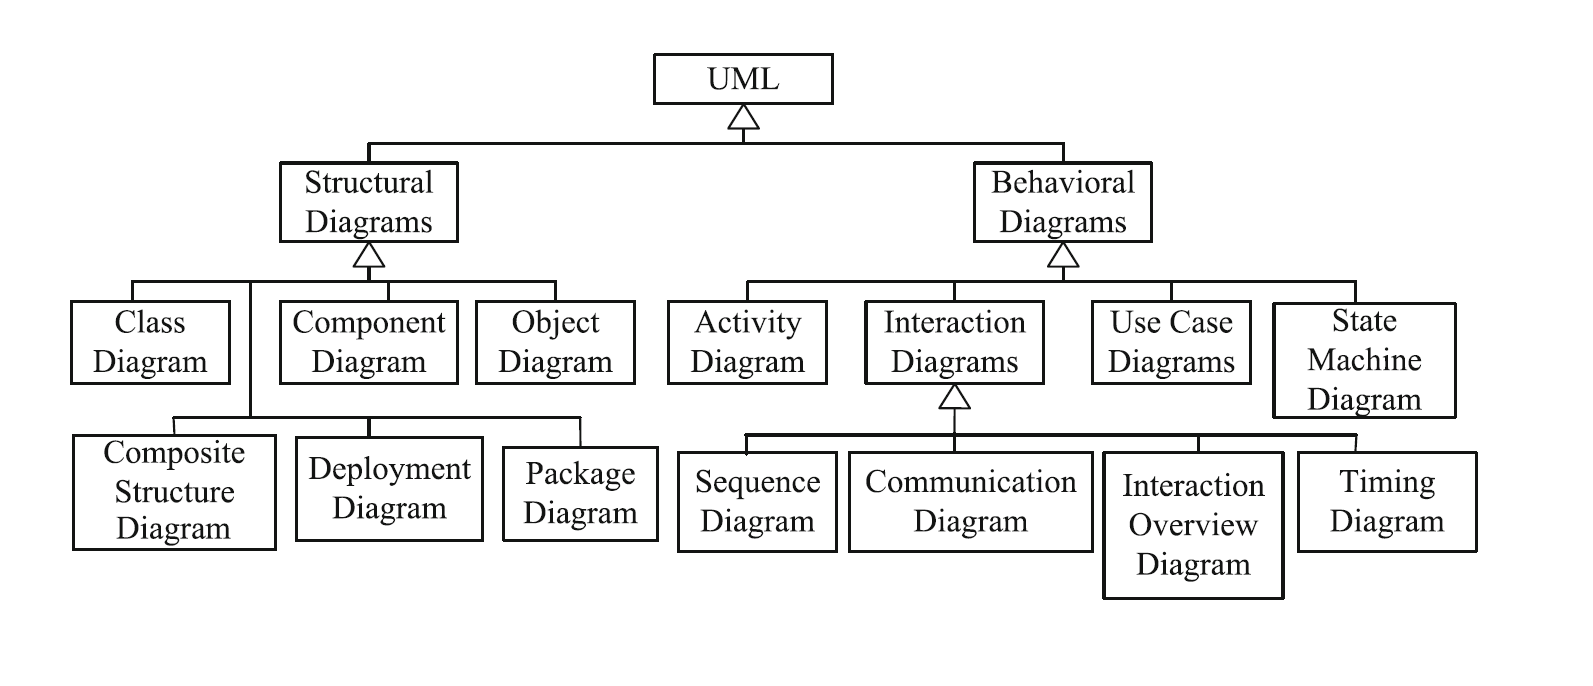
\includegraphics[scale=0.45]{figures/UML.png}
\caption{Taxonomie des diagrammes UML}
\label{UML_diag}
\end{center}
\end{figure}



\subsubsection{Profil UML}

 UML définit un concept de profil spécifique qui fournit un mécanisme d'extension générique pour construire des modèles UML dans un domaine particulier. Le profilage UML permet un affinage de la sémantique des éléments UML standard d'une manière strictement additive et sans introduire de contradictions sémantiques.
Les principaux mécanismes de profilage UML sont les stéréotypes et les valeurs marquées. Ces mécanismes sont appliqués à des éléments de modèle spécifiques tels que les classes, les attributs, les opérations et les activités afin de les adapter à différentes fins. Les mécanismes sont définis comme suit :

\begin{itemize}[label=\textbullet, font=\LARGE]
\item Les stéréotypes UML sont utilisés pour étendre le vocabulaire UML en créant de nouveaux éléments de modèle dérivés des existants. Les stéréotypes ajoutent des propriétés spécifiques adapté à un domaine de problème spécifique et sont utilisés pour la classification ou le marquage des blocs de construction UML.

\item Les valeurs marquées sont utilisées pour spécifier des valeurs de mot-clé. Elles permettent l'extension des propriétés d'un bloc de construction UML et la création de nouvelles informations dans la spécification d'un élément défini pour des éléments de modèle existants ou pour stéréotypes individuels. De plus, des valeurs balisées peuvent être utilisées pour spécifier des propriétés qui sont pertinentes pour la génération de code ou la gestion de la configuration.
Divers profils UML ont été émis par l'OMG afin de personnaliser UML pour des domaines particuliers (par exemple, l'aérospatiale, la santé, la finance, les transports, l’ingénierie des système) ou des plates-formes (par exemple, J2EE, .NET).
\end{itemize}


\subsection{SysML}

 Le langage de modélisation des systèmes (SysML) est un langage dédié aux applications d'ingénierie des systèmes. C'est un profil UML qui non seulement réutilise un sous-ensemble d'UML 2.1.1 mais fournit également des extensions supplémentaires pour mieux s'adapter aux besoins spécifiques de l'ingénierie des systèmes. 

Il est destiné à aider à spécifier et structurer des systèmes complexes et de leurs composants afin de permettre leur analyse, conception, vérification et validation. Ces systèmes peuvent être constitués de composants hétérogènes tels que du matériel, des logiciels, des informations, des processus, du personnel et des installations.
SysML englobe des capacités de modélisation qui permettent de représenter les systèmes et leurs composants en utilisant
\begin{itemize}[label=\textbullet, font=\LARGE]
\item composition, classification et interconnexion des composants structuraux;
\item les comportements, notamment les flux d'activité, les scénarios d'interaction et la transmission de messages ainsi que les comportements réactifs dépendants de l'état;
\item l'allocation d'un élément d’un modèle à un autre, comme les fonctions aux composants, composants logique aux composants physiques et logiciels au matériel; (besoin de plus de clarté)
\item les contraintes sur les valeurs de propriété du système telles que la performance, la fiabilité et les propriétés physiques;
\item les hiérarchies et les dérivations ainsi que leurs relations avec d'autres éléments  du modèle.
\end{itemize}

\subsubsection{Les quatre piliers de SysML}

 Sur  le  plan  des  concepts,  le  langage  SysML  repose  sur  quatre  ensembles  fondamentaux,  qui constituent 
les quatre piliers de SysML illustrés ci-dessous (Fig \ref{4pilliars}) :

\begin{itemize}[label=\textbullet, font=\LARGE]
\item La  notion  de  structure.  Pour  représenter  la  structure,  on  utilise  la  notion  de  bloc,  qui 
permet  de  modéliser  tout  élément  concret  :  système,  sous  systèmes,  composants logiciels  ou  matériels,  mais  aussi  acteurs,  système  externes,  ou  encore  éléments  de 
matière, d’énergie ou d’information échangés.  Les diagrammes correspondants sont les diagrammes de définition de bloc et de bloc interne ;
\item La notion de comportement, pour la modélisation dynamique ou comportementale du système  ou  d’un  constituant.  Les  diagrammes  correspondants  sont  les  diagrammes d’activités et d’états (et au besoin de séquence);
\item La notion d’exigence. Le diagramme correspondant est le diagramme d’exigences ;
\item Les  équations  et  contraintes  régissant  le  système  ou  ses  constituants.  Le  diagramme correspondant est le diagramme paramétrique.


\end{itemize}

\begin{figure}[H]
\begin{center}
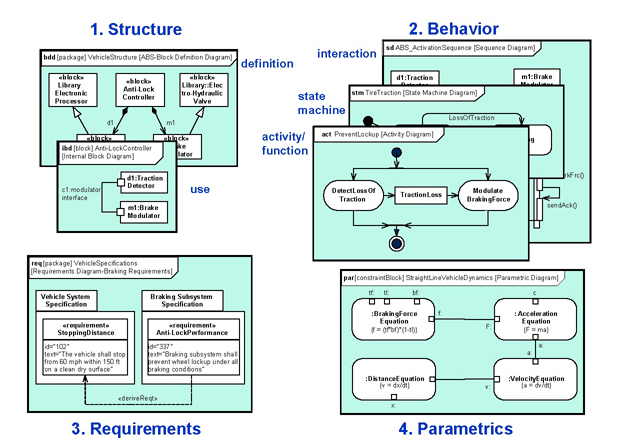
\includegraphics[scale=0.75]{figures/4pillars.png}
\caption{Les quatre piliers de SYSML}
\label{4pilliars}
\end{center}
\end{figure}

\subsubsection{Architecture SysML}

 Les diagrammes SysML définissent une syntaxe concrète qui décrit comment les concepts SysML sont visualisé graphiquement ou textuellement. Dans la spécification SysML, cette notation est décrite dans des tableaux qui montrent la cartographie des concepts de langage en symboles graphique sur les diagrammes. La taxonomie des diagrammes est illustrée à la Fig \ref{SysML_diag}.

SysML réutilise complètement certains diagrammes de UML 2.1:
\begin{itemize}[label=\textbullet, font=\LARGE]
\item Cas d'utilisation
\item Séquence
\item État machine
\item Package
\end{itemize}
En outre, deux nouveaux diagrammes sont ajoutés :
\begin{itemize}[label=\textbullet, font=\LARGE]
\item Exigences
\item Paramétrique
\end{itemize}
De plus, d'autres diagrammes UML sont réutilisés sous forme étendue :
\begin{itemize}[label=\textbullet, font=\LARGE]
\item Activité (étend le diagramme d'activité UML)
\item Définition de bloc (étend le diagramme de classes UML)
\item Bloc interne (extension du diagramme de structure composite UML)
\end{itemize}

\begin{figure}[H]
\begin{center}
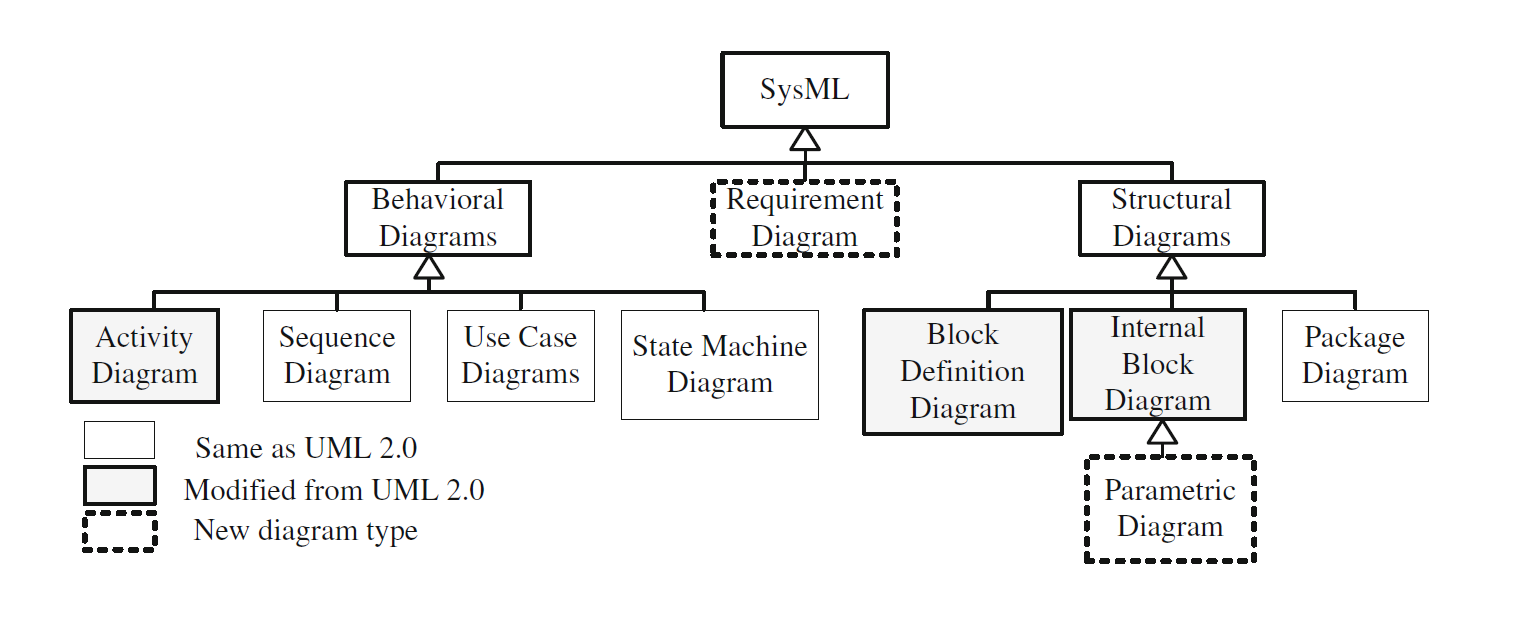
\includegraphics[scale=0.45]{figures/SysML.png}
\caption{Taxonomie des diagrammes SysML}
\label{SysML_diag}
\end{center}
\end{figure}

\subsubsection{La relation entre UML et SYSML}

 SysML réutilise un sous-ensemble de UML 2.1, appelé "UML4SysML", qui représente environ la moitié du langage UML. Une partie importante de l'UML des concepts ont été écartés car ils n'étaient pas considérés comme pertinents pour les besoins du modèle de SE.
Certains des diagrammes réutilisés ont été inclus comme dans UML 2.1.1 .
Ceux-ci incluent la machine d'état, la séquence et les diagrammes de cas d'utilisation.
D'autres diagrammes ont été étendus, tels que les diagrammes d'activité, afin de répondre aux besoins spécifiques des SE.
De plus, SysML a omis certains diagrammes UML, à savoir d'objet, de composant, de déploiement,de communication, de temps et d'interactions.
Les diagrammes de structure dont diagramme de Classe et composition ont été fondamentalement modifiés et remplacés par des diagrammes de définition de blocs et diagrammes de blocs internes. Ces extensions sont basées sur le mécanisme de profilage UML standard, qui inclut les stéréotypes UML, extensions de diagramme UML et la bibliothèques de modèles. Le mécanisme de profilage a été choisi sur d'autres mécanismes d'extension afin de tirer parti des outils existants basés sur UML pour la modélisation de systèmes. En outre, SysML ajoute deux nouveaux diagrammes, ceux-ci étant diagrammes d'exigences et diagrammes paramétriques, et intègre de nouvelles capacités de spécification liens tels que l'allocation. La relation entre UML et SysML est illustrée dans \ref{relationUS}.


\begin{figure}[H]
\begin{center}
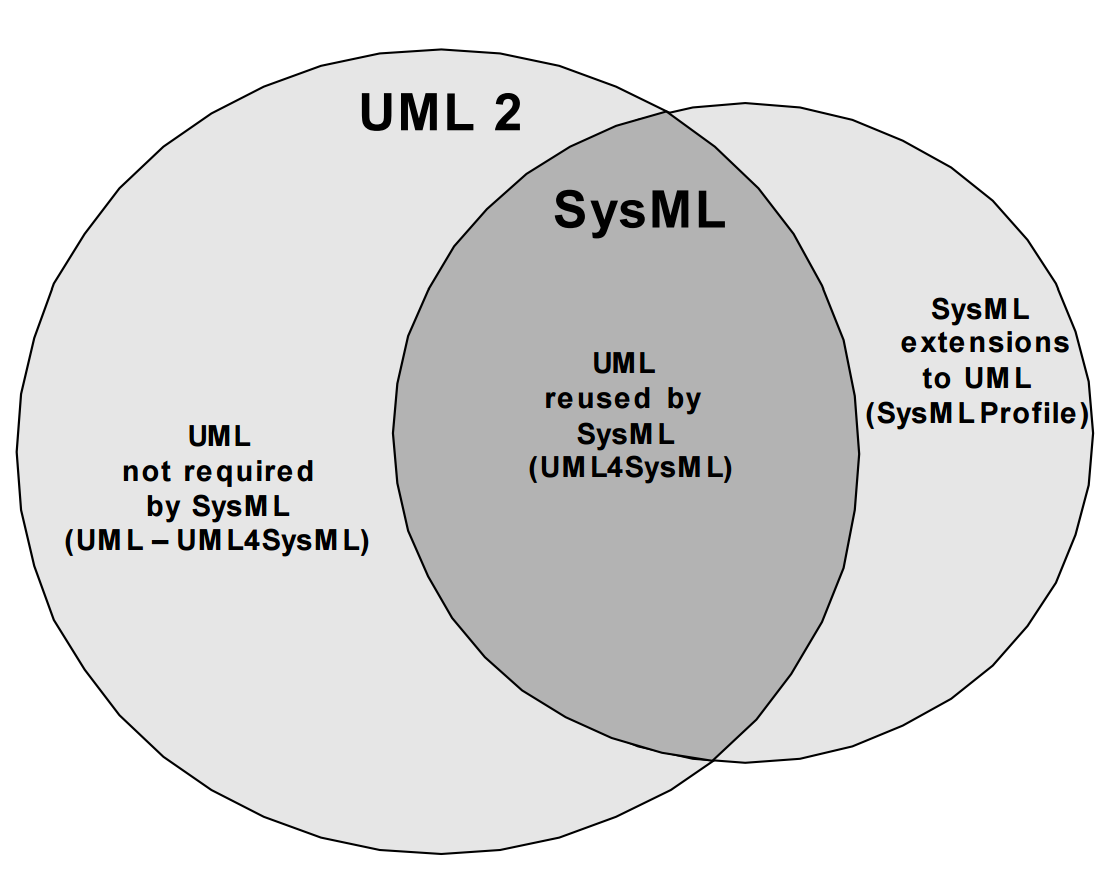
\includegraphics[scale=0.2]{figures/relationshipUS.png}
\caption{La relation entre UML et SYSML}
\label{relationUS}
\end{center}
\end{figure}

\section{Automates temporisés}

 Les automates temporisés reprennent
le formalisme des automates auxquels s’ajoutent des horloges. Dans le formalisme des automates, un système est représenté par un ensemble de sommets décrivant les états du système, ces sommets étant reliés par des arcs étiquetés par des événements.
Dans un automate temporisé, la dynamique temporelle est décrite grâce aux horloges qui permettent la définition de contraintes temporelles associées aux sommets ou aux
arcs. Une contrainte temporelle associée à un sommet est appelée son invariant, celle associée à une transition est nommée une garde. Il est possible de rester dans un état
aussi longtemps que son invariant est vrai. Une transition peut être déclenchée dès que sa garde est vraie. Lors de l’exécution d’une transition, la remise à zéro des horloges
est possible.
On note $\mathcal{\phi}$($\mathcal{X}$) l’ensemble des contraintes d’horloges. Un automate temporisé est défini par un n-uplet $\mathcal{<}$
$\mathcal{S}$, $\mathcal{X}$, $\mathcal{L}$, $\mathcal{E}$, $\mathcal{I}$ $\mathcal{>}$ où :

\begin{itemize}
\item  $\mathcal{S}$ est un ensemble fini de sommets,$s_{0}$ 
$\mathcal{\in}$  $\mathcal{S}$ étant le sommet initial ;

\item  $\mathcal{X}$ est un ensemble fini d’horloges ;

\item  $\mathcal{L}$ est un ensemble fini d’étiquettes ;

\item  $\mathcal{E}$ est un ensemble fini d’arcs ; chaque arc
$e_{ }$ est un n-uplet ($s_{ }$, $l_{ }$, $\varphi$, $\delta$, $s'_{ }$) tel que $e_{ }$ relie $s_{ }$ $\mathcal{\in}$  $\mathcal{S}$, état source, à $s'_{ }$ $\mathcal{\in}$  $\mathcal{S}$, état destination, et est étiqueté par l’événement $l_{ }$ ;
la condition d’activation que doit satisfaire les horloges pour franchir la transition est représentée par la contrainte temporelle $\varphi$ $\mathcal{\in}$ $\mathcal{\phi}$($\mathcal{X}$),$\delta$ $\subseteq$ $\mathcal{X}$ correspond à l’ensemble des horloges réinitialisées lorsque la transition est tirée ;

\item $\mathcal{I}$ : $\mathcal{S}$ $\rightarrow$ $\mathcal{\phi}$($\mathcal{X}$) associe à chaque sommet de l’automate temporisé une contrainte temporelle appelée l’invariant du sommet.

\end{itemize}

 La théorie des automates temporisés permet de décrire un système complexe comme un produit d’automates, ce qui autorise la construction modulaire du système global. Chaque automate décrit un sous-système et la synchronisation entre les automates se fait par le biais d’événements de synchronisation. Lors de la définition des composants, il est alors nécessaire de distinguer les événements internes décrivant la dynamique propre et asynchrone du sous-système, des événements externes qui provoquent l’évolution simultanée de tous les sous-systèmes partageant ces événements.


\section{Ingénierie dirigée par les modèles - IDM}
\subsection{Définitions}
\subsection{Transformation des modèles}
\subsubsection{Transformation Model to Model - M2MT}
\subsubsection{Transformation Model to Text  - M2TT}

\section{Modélisation des systèmes complexes}
 Dans cette partie, nous présentons des défis pour l'intégration et l'évaluation de la différence entre les techniques de spécification semi-formelles et formelles. En outre, nous présentons plusieurs formalismes de spécifications, des similitudes et des différences, ainsi que des possibilités de combiner de telles techniques. Le premier aspect critique du développement de logiciels basés sur les composants est la spécification qui décrit la fonctionnalité et le comportement du composant.
\subsection{Langage Naturel}
Un langage naturel (LN) n’est pas non formel en lui-même. Il est défini par un ensemble de règles (de grammaire) et sur un vocabulaire fini bien que très large. Néanmoins, ce vocabulaire est évolutif et les pratiquants  d’une  langue  ne  s’accordent  pas  toujours  sur  les  règles grammaticales à respecter (ou à appliquer) ni sur la sémantique qui leur est associée.
Le  langage  naturel  est  le  langage  qui  est  parlé  ou  écrit  (français,anglais  ...)  pour  communiquer.  Tout  langage  naturel  est  facilement utilisable  et compréhensible  par  un  humain  parlant  ce  langage,  ce
qui  en  fait  le  moyen  le  plus  simple  et  direct  pour  communiquer  et exprimer ses besoins ou la perception d’un problème.
Le langage naturel est sans doute le langage le plus expressif. 
Son écriture donne la possibilité d’exprimer une même idée en la formulant  de  différentes  manières  et  d’avoir  pour  une  même  formulation plusieurs sens.  Cela  peut  donner  lieu  à  des  problèmes  de  communication  dus  à  des  interprétations  multiples.  La  compréhension  du
sens d’un énoncé demande parfois au lecteur, un effort d’interprétation ou d’inférence en fonction d’un contexte particulier.
La compréhension du sens fait souvent appel à des connaissances implicites et extérieures à l’énoncé. En outre, dans le cas d’une collaboration en domaine pluridisciplinaire, la terminologie utilisée peut différer et donc poser des problèmes de communication et de compréhension.
La richesse des langages naturels, ainsi que l’interprétation variable du  sens  terminologique  et  grammatical  des  formulations  possibles font  que  les  spécifications  écrites  en  langage  naturel  sont  connues pour  être  ambiguës.  Les  spécifications  LN  sont  aussi  connues  pour pouvoir  véhiculer  des  informations  pertinentes  de  façon  implicite.
Dans ce cas, l’appel à des connaissances extérieures aux textes ainsi qu’un effort de déduction sont nécessaires pour la compréhension de la spécification et peuvent malgré tout conduire à une mauvaise interprétation.
Du fait de leurs ambiguïtés et de leur contenu implicite, les spécifications en LN posent le problème d’être difficilement interprétables par une machine. Il n’est donc pas possible d’effectuer de manière directe une vérification automatique prenant ce genre de spécification en entrée.




\subsection{Langage Semi-Formel}
\subsection{Langage Formel}

\section{Vérification et Validation}

\subsection{Test et Simulation (Validation)}

 Le test consiste à effectuer des actions spécifiques afin de vérifier l'opérabilité,capacité de support ou capacité de performance d'un article lorsqu'il est soumis à des conditions contrôlées réelles ou simulées. Les résultats obtenus sont ensuite comparés à ceux prévus ou attendus. Cela implique souvent l'utilisation d'un équipement d'essai spécial ou instrumentation afin d'obtenir des données quantitatives précises pour l'analyse.
bien que les tests soient bien connus et aient été largement utilisés dans le génie logiciel,ils permettent seulement la découverte tardive des erreurs, et certains types d'erreurs peuvent effectivement rester transparent.

 La simulation est  la  méthode traditionnelle  de  vérification.  Comme  son  nom l’indique,   elle    essaye   de tester   le   bon fonctionnement    d’un    composant    en    le soumettant   à  un   système   réel   d’évaluation. Clairement  le  succès    de  cette  technique  compte beaucoup    sur  la  détermination  et  l’attachement de  l’individu  qui  fait  le  contrôle.  Aussi  chaque fois  qu'un  changement  est  fait  au  code  HDL (Hardware Description Language) on a besoin du même   effort   pour   vérifier   la   simulation résultante.  Mais,  bien  que  la  technique  standard de  vérification  soit  le  test  direct,    cette  méthode permet d’afficher la présence d’erreurs mais n’est pas  capable  de  prouver  avec  certitude  leur absence.  Cette  conclusion  découle  de  plusieurs arguments dont figure principalement l’impossibilité   d’énumérer   toutes   les   entrées possibles.  

\subsection{Méthodes Formelles (Vérification)}

 La vérification formelle    est un processus [3] qui   permet   de   prouver   qu’un   système   se 
Comporterait    en    parfait    accord    avec    sa spécification.   Cela   revient   à   utiliser   des approches mathématiques qui permettent de montrer   que   l’implémentation   satisfait   la  
Spécification. Dans ce cas une considération de tous les cas possibles est implicite. Ces dernières années, les méthodes formelles ne sont plus uniquement des thèmes de recherche, mais plutôt un concurrent potentiel, si ce n’est pas une solution de remplacement, de la vérification par simulation. Ces points de vue partent d’une correcte énumération des caractéristiques des méthodes formelles. Les avantages des méthodes de vérification formelle comparées à la vérification par simulation sont nombreux. En effet, ces méthodes considèrent toutes les entrées possibles au système, vérifient la validité des propriétés du système mathématiquement, ne nécessitent pas une spécification des sorties du système prévue de plus elles permettent, pour certains outils, d’identifier les traces des erreurs s’il y a lieu. La vérification formelle possède, elle 
Aussi, certains inconvénients [3]. En effet, elle demande un effort supplémentaire pour parvenir à une description complète et simple du système à vérifier. C’est qu’il est nécessaire de définir une spécification, d’une part, tenant en considération tous les détails du système, et d’autre part, assez simple à manipuler dans la phase de vérification. D’autre part c’est difficile de faire un raffinement sans perte des propriétés du système. 

\subsubsection{Model-checking}

 Issu du domaine des méthodes formelles, le model-checking (Clarke et al., 2002) est utilisé pour la vérification automatique de systèmes complexes représentés par des
systèmes à événements discrets. Lorsque le modèle d’un système est décrit sous la forme d’un automate temporisé, les propriétés sont exprimées à l’aide d’une logique temporelle. Le problème du model-checking peut alors se résumer de la façon suivante : étant donné M un modèle du système et
$\varphi$ une propriété à vérifier, est-ce que M satisfait $\varphi$ ? Les programmes de model-checking retournent une réponse binaire (la propriété $\varphi$ est vérifiée ou ne l’est pas).
La logique la plus répandue pour la vérification d’automates temporisés est la logique TCTL (Timed Computation Tree Logic) qui est une extension de la logique CTL autorisant l’expression de contraintes temporelles dans les propriétés. Les formules TCTL sont définies de manière inductive par la grammaire suivante définie dans (Henzinger et al., 1994) :

\centerline{$f_{ }$ ::= $p_{ }$ $|$ $x_{ } \in \mathcal{I}$ $|$ $\neg f_{ }$ $|$ $f_{1} \vee f_{2}$ $|$ $\exists \diamondsuit_{I} f_{ } $ $|$ $\forall \diamondsuit_{I} f_{ } $}
avec $p_{ } \in P$ un prédicat de base,$x_{ } \in X $  une horloge et I un intervalle de temps.

On trouve les abréviations $\forall \Box f_{ }$ pour $\neg \exists \diamondsuit \neg f_{ }$ et $\exists \Box f_{ }$ pour $\neg \forall \diamondsuit \neg f_{ }$. Intuitivement
l’opérateur $\exists \diamondsuit_{I} f_{ }$ signifie qu’il existe une exécution menant à un état satisfaisant la
propriété $f_{ }$ au temps $t \in I$.
$\forall \diamondsuit_{I} f_{ }$ signifie que chaque exécution possède un état où la propriété $f_{ }$ est valide au temps $t \in I$.
$\forall \Box f_{ }$ signifie que tous les états sur tous les
chemins d’exécution satisfont la propriété $f_{ }$.
$\exists \Box f_{ } $ signifie qu’il existe une exécution
telle que tous les états sur le chemin d’exécution satisfont la propriété $f_{ }$.

Un automate temporisé ayant la particularité de posséder un nombre infini de comportements liés à la valuation de ses horloges, on se trouve confronté au problème
de l’explosion combinatoire. Afin de résoudre ce problème, le model-checking symbolique représente des ensembles d’états à l’aide de structures de données efficaces
comme les diagrammes de décision binaire (encore appelés BDD pour Binary Decision Diagram), ou les matrices de bornes (DBM pour Difference Bound Matrices).
Les algorithmes de model-checking symboliques travaillent sur ces ensembles d’états et déterminent, en fonction des propriétés à vérifier, soit l’espace atteignable, soit l’ensemble des états satisfaisant une formule TCTL (Berard et al., 2001).

\paragraph{Langage de description UPPAAL}

 Les outils les plus connus pour le model-checking symbolique sur les automates temporisés sont KRONOS (Yovine, 1997) et UPPAAL (Larsen et al., 1997). Ce dernier régulièrement mis à jour par de nouvelles fonctionnalités et disposant d’une interface graphique agréable a été utilisé pour la réalisation de cette étude. UPPAAL étend le formalisme des automates temporisés présenté précédemment par de nouvelles caractéristiques et des notations particulières. La première extension concerne la définition possible de variables entières pouvant être associées à des états et modifiées lors du déclenchement de transitions. La seconde évolution touche à la synchronisation d’automates réalisée par le biais de canaux de synchronisation. Par exemple avec UPPAAL les notations a! et a? représentent respectivement des événements émis et reçus sur le canal a. Dans le système global, produit synchronisé de tous les automates, à chaque événement reçu doit correspondre un événement émis alors que les transitions
non synchronisées correspondent à une évolution asynchrone du sous-système.

\subsubsection{Theorem Proving}

 Theorem Proving implique de vérifier la véracité des théorèmes mathématiques qui sont postulés ou inférés tout au long de la conception en utilisant un langage de spécification formelle. La procédure suivie pour prouver de tels théorèmes implique généralement deux composants principaux, à savoir un vérificateur de preuve et un moteur d'inférence. Cependant, alors que le premier peut être complètement automatisé dans la plupart des cas, le second peut exiger un guidage humain occasionnellement, empêchant ainsi l'automatisation de l'ensemble du processus.
 De plus, il peut y avoir de rares cas où en raison du formalisme impliqué (par exemple, des références cachés circulaires conduisant à un paradoxe logique),la conjecture d'un théorème donné ne peut être ni prouvé ni réfuté. Les problèmes mentionnés ci-dessus représentent certaines des principales raisons pour lesquelles il n'est actuellement pas largement adopté pour effectuer la vérification et la validation.


\part{Chapitre 2}
\chapter{Approche}
Vers une Vérification Formelle des Modèles SYSML

\part{Chapitre 3}
\chapter{Séquence Formel : Génération d'automates de vérification}
\subsection{De SYSML vers UPPAAL}
\subsection{Algorithmes développer}
\subsection{Étude de cas}

\chapter{Conclusion et Futur Travaux}

\end{document}
